%% Based on <bare_jrnl.tex> in the ieee package available from CTAN,
%% I have changed the options so that most useful ones are clubbed together,
%% Have a look at <bare_jrnl.tex> to understand the function of each package. 

%% This code is offered as-is - no warranty - user assumes all risk.
%% Free to use, distribute and modify.

% *** Authors should verify (and, if needed, correct) their LaTeX system  ***
% *** with the testflow diagnostic prior to trusting their LaTeX platform ***
% *** with production work. IEEE's font choices can trigger bugs that do  ***
% *** not appear when using other class files.                            ***
% Testflow can be obtained at:
% http://www.ctan.org/tex-archive/macros/latex/contrib/supported/IEEEtran/testflow

%        File: 200801011.tex
%     Created: Mon Apr 16 03:00 PM 2012 I
% Last Change: Mon Apr 16 03:00 PM 2012 I
%
\documentclass[conference]{IEEEtran}

\usepackage{cite, graphicx, subfigure, amsmath, algpseudocode, float} 
\usepackage[bookmarks=true,colorlinks=false,pdfborder={0 0 0}]{hyperref}
\renewcommand{\algorithmicrequire}{\textbf{Input:}}
\renewcommand{\algorithmicensure}{\textbf{Output:}}
\interdisplaylinepenalty=2500

% *** Do not adjust lengths that control margins, column widths, etc. ***
% *** Do not use packages that alter fonts (such as pslatex).         ***
% There should be no need to do such things with IEEEtran.cls V1.6 and later.


% correct bad hyphenation here
\hyphenation{}


\begin{document}
%
% paper title
\title{Semantic mapping of XML metadata on the Cloud}
%
% author names and IEEE memberships
\author{\IEEEauthorblockN{Nikhil Marathe}
\IEEEauthorblockA{
    Dhirubhai Ambani Institute of Information and Communication Technology\\
    Gandhinagar, Gujarat - 382007\\
    \texttt{200801011@daiict.ac.in}
}
\emph{Supervisor}\\\emph{Dr. Sourish Dasgupta}
}% <-this % stops a space
%

% make the title area
\maketitle

\begin{abstract}
    We propose a system for conversion of XML data from heterogenous services
    into structured data with semantic information and its storage in
    a distributed manner. The system implements a triplestore over
    a distributed key-value store using a unique graph mapping of ontologies to
    allow fast retrieval.
\end{abstract}

\begin{IEEEkeywords}
    Distributed databases, Query processing, Schema and sub-schema, Data
    mining, Knowledge management applications, Web mining, RDF, Semantic web.
\end{IEEEkeywords}

\section{Introduction}
\IEEEPARstart{T}{he} semantic web has made significant strides in the recent
past. The Linked Data initiative aims to make graph structured data encoded in
RDF and available over HTTP. Still there remains a significant portion of data
that is unstructured or semi-structured but contains valuable information. An
example of this is microformats\cite{Khare:06} embedded in web pages or the
various formats used by social networks to publish various messages about the
activity of their members. This information is not available in a semantically
aware form due to various reasons. For example, the micro-blogging website
Twitter produces
340 million tweets
a day\footnote{http://blog.twitter.com/2012/03/twitter-turns-six.html}.
This data is available in custom XML format. Similarly various scientific
sensors around the world constantly produce data. The rate of data
production on the Internet is sky-rocketing, and storage and analysis of
this data has become a new computing problem under the moniker of Big Data.
This paper makes the following contributions:

\begin{itemize}
    \item Provides an attempt at translating XML data to structured RDF data.
    \item Presents a conversion of ontology data to a cached 'Clusterspace' to
        allow fast, distributed reads.
    \item Storage of RDF data over a distributed key-value store and the
        problem that occurs in real implementation.
\end{itemize}

\section{Background}
\label{sec:background}


TODO: diff between XML and RDF

\section{System}
Our system has the following core modules (see Figure \ref{fig:architecture}):

\begin{itemize}
    \item \emph{Clusterspace} - A graph of the various concepts spanning all
        known ontologies.
    \item \emph{Triple store} - An RDF triple store implemented over Apache
        Cassandra\footnote{http://cassandra.apache.org}.
    \item \emph{XML to RDF converter} - Attempts to generate a set of RDF
        triples from semantic information extracted from XML data.
\end{itemize}

\begin{figure*}
    \centering
    \includegraphics[scale=0.5]{images/architecture}
    \caption{System architecture}
    \label{fig:architecture}
\end{figure*}

\emph{Publishers} feed data to the system via XML or RDF. The Clusterspace is
built up as and when new ontologies are introduced to the system. Information
from the Clusterspace and the input data is used to store triples.
\emph{Subscribers} may then query the system to obtain RDF output of all known
data in the database via the SPARQL interface.

\subsection{Clusterspace}
The Clusterspace is a graph representation of a subset of the axioms stated by
all known ontologies. The Clusterspace is built up by using a \emph{reasoner}
TODO:which? the first time an ontology is introduced to the system. 

The Clusterspace stores two distinct directed trees. One is the Class heirarchy
and the other is the Property heirarchy. As new ontologies are introduced, the
reasoner is used to find the appropriate position to insert the class
(\texttt{rdf:Class}) in the Class heirarchy. The Class heirarchy has as its
roots the classes that have no super-classes. We choose not to deal with
\texttt{owl:Thing} as the single root unless an ontology explicitly introduces
it. The Property heirarchy is similar but uses the \texttt{rdf:subPropertyOf}
relationship to infer the heirarchy.

The class heirarchy also encodes object properties. An edge is created from the
domain of the property to the range(s). For datatype properties, all ranges are
co-erced to the string representation, with only
\texttt{string}\footnote{http://www.w3.org/2001/XMLSchema\#string} existing in
the Clusterspace.

The full algorithm for forming the clusterspace can be found in \ref{cs-algo}.
The advantages and limitations of building up a Clusterspace are:

\subsubsection*{Advantages}
\begin{itemize}
    \item Fast lookup of known classes using exact or approximate matches.
    \item Reasoning only has to be performed once, after that only simple graph
        traversal is required.
    \item Clusterspace can be shared and updated across a distributed system.
\end{itemize}

\subsubsection*{Limitations}
\begin{itemize}
    \item The Clusterspace does not encode full reasoning information.
    \item Complete RDFS entailment support is not currently implemented. (For
        example, relationship transitivity is not implemented yet.)
    \item Datatype information for the range is lost on Datatype Properties.
\end{itemize}

Once the Clusterspace has been extended with some ontology, queries over that
ontology can be augmented with entailment. For example, the query:

\begin{verbatim}
PREFIX db: <http://dbpedia.org/ontology/>
SELECT ?p WHERE {
    ?b a db:Book .
    ?p a db:Person .
    ?b db:author ?p .
}
\end{verbatim}

over \ref{fig:person-cs-example}, will return books written by actors as well
as politicians. Since a Book is a Work, property ``author'' has domain as Work
and range as Person, and Actor and Politician are subclasses of Person.

\begin{figure}
    \caption{Sample Clusterspace - DBpedia Work and Person}
    \label{fig:person-cs-example}
\end{figure}

\subsection{XML to RDF conversion}

The current implementation of the XML to RDF conversion takes a very naive
approach to extracting information from the XML data. It can be immensely
augmented by using statistical properties and methods from Information
Retrieval.

The fundamental difference between plain XML and semantic data is explained in
section~\ref{sec:background}. For example consider
document~\ref{ex:xml-rec}\footnote{Based on the Music Ontology
- http://purl.org/ontology/mo/}. Here it is quite evident to a human that
Record ``OK Computer'' contains the track ``Paranoid Android'' of duration
384000ms. We use the known data properties of tags found in the data to figure
out if a datatype property reference can be resolved to a known instance
specified somewhere else in the document. We observe that the value of
a datatype property and the type of a instance can uniquely identify the
instance we are referring to\footnote{Although multiple instances can have the
    same value of a datatype property, e. g. \texttt{Person} having
    \texttt{age}, we assume that an XML representation will not use
a non-injective property to refer to instances}. Hence our lookup table is
a mapping from $(type, value)\rightarrow instance$. Although our algorithm
accepts plain XML, it has some preconditions for it to work:

\begin{itemize}
    \item The tag names should be class or property names from a known ontology.
    \item Attribute names should be a datatype property name from an known
        ontology.
    \item The top level tags should be class names.
    \item The conversion considers only one level of nesting in associating
        data. For example, in document~\ref{ex:xml-bad} it won't infer that the
        artist is called Radiohead.
\end{itemize}

Since these datatype property based references can be present after their use
(in terms of sequential bytes), unresolved references have to be maintained
until the entire document has been parsed, which are then resolved to create
a set of RDF triples. Based on our assumption that the top level tags are class
names, we find the right class in the clusterspace from the tag name. In case
of multiple possibilities, the implementation currently chooses the first one.
This allows us to know what properties may be defined by the inner tags. If
there are no inner tags or attributes, this XML node is itself a reference.
Otherwise this node maps to a new RDF subject instance with the
rdf:type\footnote{http://www.w3.org/1999/02/22-rdf-syntax-ns\#type} as the
class found for the tag name.

All attributes can only be datatype property instances, so we use the attribute
name to lookup the datatype property and the attribute value as the value for
this instance. A child tag can be:
\begin{enumerate}
    \item \emph{A datatype property} - In this case the child element can only
        have text content. This gives us information about the current instance
        and is added to the lookup table. A triple is also created.
    \item \emph{An object property} - If the child has only text, then the
        object in the $(subject, property, object)$ triple is a reference. This
        reference can be from any of the classes in the range of the object
        property. If the child has tags then each of those tags are treated as
        a possible description of an instance and parsed recursively. TODO:
        mention using statistics to deal with a tag defined only by its
        properties.
    \item \emph{A class} - In this case the tag is defining an instance or
        reference. Based on the known object properties, our system attempts to
        find possible object properties on the $subject$ that have the class in
        their range. The first of these is picked to create the triple.
\end{enumerate}

\begin{figure}
    \caption{Example XML document.}
    \label{ex:xml-rec}
    \begin{verbatim}
    <Track>
        <title>Paranoid Android</title>
        <duration>384000</duration>
    </Track>
    <Record title=``OK Computer''>
        <track>
            Paranoid Android
        </track>
    </Record>
    \end{verbatim}
\end{figure}

\begin{figure}
    \caption{Bad XML}
    \label{ex:xml-bad}
    \begin{verbatim}
    <MusicArtist>
        <Record>
            <title>OK Computer</title>
            <name>Radiohead</name>
        </Record>
    </MusicArtist>
    \end{verbatim}
\end{figure}

\subsection{Storing RDF in Cassandra}

Apache Cassandra\footnote{http://cassandra.apache.org} is a distributed,
column-oriented, eventually-consistent database, based on the Google
Bigtable\cite{Chang06bigtable:a} and Amazon
Dynamo\cite{Hastorun07dynamo:amazon's} systems. It provides a non-relational
key-value database with replication and partitioning across a cluster. Using
the concept of super-columns, Cassandra also allows a two-level hash table,
${ key1 : { key2 : value } }$.

TODO: What is Cassandra and Why Cassandra?

The Cassandra data model allows nested storage using super columns. We use the
approach described by Ladwig and Harth\cite{ladwig:11}, but only maintain two
models - SPO and OPS. In SPO each subject instance is a row key, the predicate
name is the supercolumn key and each object is one column. The OPS index is
used for performance improvements. We provide two additional Column-families in
our system.

\begin{enumerate}
    \item \emph{Concepts} - Each row is the full IRI of a class from the known
        ontologies. Every column is the IRI of an instance of that class. In
        addition instances of subclasses are also stored for the class.

    \item \emph{InstanceData} - Since our system is designed for data mining,
        the SPARQL response is not simply a set of triples, but full RDF dumps
        for each subject of the triples in the final result. To prevent having
        to iterate over all of an instances properties every time, a complete
        RDF/XML representation of every instance is kept in this column family,
        indexed by the IRI of the instance.

\end{enumerate}

TODO: graphic of columnfamilies

\section{Evaluation}

The implementation of the system was done in Java and run on JVM version 1.6. The main
process was run with a maximum heap size of 2G and a start heap size of 1G.

The actual implementation uses the following libraries:
\begin{enumerate}
    \item Neo4j\footnote{http://neo4j.org} for the Clusterspace.
    \item Apache Cassandra\footnote{http://cassandra.apache.org} for the data storage.
    \item OWLAPI\cite{Hor:09} for handling ontologies.
    \item Apache Jena\footnote{http://incubator.apache.org/jena/} for SPARQL and RDF parsing.
    \item JDOM\footnote{http://jdom.org} for XML parsing.
    \item Pellet\cite{Parsia04pellet:an} as the DL-reasoner.
\end{enumerate}

We performed performance evaluations for our system in four parts.

For all tests, the hardware was a 2011 Macbook Pro with Snow Leopard 10.6.8,
2.3GHz Intel Core i7, 8GB RAM, and a 7200rpm Hard Drive.  JVM 1.6.0 was used.
  The start heap size for the system was 1G, for Cassandra it was 400M. Max
  heap size for the system was 2G, for Cassandra it was 4G.

For the distributed Cassandra test a cluster of 4 nodes on Amazon
EC2\footnote{TODO} was used.  Each machine had 8GB of RAM, out of which
Cassandra was allocated 4GB. One of the nodes ran our system. TODO processors on each?
+ OS.

The dataset used for the data loading and queries was generated by the LUBM \texttt{ubt} generator tool. LUBM provides 14 queries to measure the performance of a system. Queries 11, 12 and 13 are not applicable to the system as it does not perform full RDFS entailment yet. Queries 2, 7 and 9 would either timeout or the Jena SPARQL processor would run out of memory and halt, hence these queries have not been performed.

\subsection{Loading an ontology in the clusterspace}

\subsubsection{Time for class heirarchy formation}

The DBpedia ontology v3.6 has 272 classes, 629 object properties and 706
datatype properties. One of the key measures is the time taken to build the
class heirarchy. Therefore we ran runs with modified DBpedia ontologies to have
10 to 272 classes, randomly picked. 10 versions of each ontology was generated
and the time averaged. Each test itself was also run 10 times. The first
result was excluded since to allow for the data to be loaded into RAM and
then averaged.

Figure \ref{fig:eval:cs-ch-form} shows the results. As is seen, addition is
nearly linear time with the tree traversals (see Section
\ref{cs-compare-classes}) accounting for an approximately logarithmic factor.

\begin{figure}[h]
    \centering
    \includegraphics[scale=0.35]{../../graphs/full-register-random/register-classes.png}
    \caption{Class heirarchy formation time}
    \label{fig:eval:cs-ch-form}
\end{figure}

\subsection{XML to RDF conversion time}

To measure the time taken for XML to RDF conversion, a sample RDF file
generated using the LUBM data generator was used. It had 20659 class instances
and 82415 property instances. A tool which read RDF and generated random XML structures
was used to generate 10 versions of the RDF file. Each XML file was run through the converter 10 times. The test results are in Figure %\ref{fig:eval:xml2rdf} TODO: needs for different number of RDF triples :(

\subsection{Query clusterspace time}

For query processing, there are two measurements. One is the time spent traversing the clusterspace, and the other is time spent fetching data from Cassandra. The clusterspace is located only on one machine. Times measured are for the LUBM sample queries run on test data with 129533 class instances and 516116 property instances over the LUBM University Bench Ontology. Figure \ref{fig:eval:qcs} shows the time for Clusterspace traversal.

As is seen, clusterspace operations are quite fast. The main improvement over a reasoner is that for every query of every client, the reasoner may have to re-parse various ontologies and make inferences. More importantly, in a distributed system, each machine will have to run its own reasoner on its own set of ontologies. By having a shared Clusterspace, changes in data and inferences can be reflected across all machines without much of a performance hit. For simple queries in particular, the Clusterspace shows sub 10 millisecond times.

\begin{figure}[h]
    \centering
    \includegraphics[scale=0.35]{../../graphs/full-query/qm}
    \caption{Query retrieval Clusterspace traversal time}
    \label{fig:eval:qcs}
\end{figure}

\subsection{Query retrieval time}

\subsubsection{Cassandra on a single node}

TODO

\begin{figure*}[t]
    \centering
    \mbox{
        \subfigure{
            \includegraphics[scale=0.35]{../../graphs/full-query/qr}
        }
        \quad
        \subfigure{
            \includegraphics[scale=0.35]{../../graphs/cluster-query/qr.png}
        }
    }
    \caption{Query retrieval total time - a) Single node b) Cluster }
    \label{fig:eval:qtotal}
\end{figure*}

\subsubsection{Cassandra on a 4 node cluster}

inference that cassandra is a bad idea for speed, move computation to the data and all.

%\begin{figure}[h]
%    \centering
%    \includegraphics[scale=0.35]{../../graphs/full-register/register}
%    \caption{Clusterspace formation time}
%    \label{fig:eval:cs-form}
%\end{figure}
%
%\subsubsection{Total time for Clusterspace formation}
%To measure the total time, the same DBpedia ontology was used. Figure
%\ref{fig:eval:cs-form} show the test results. Adding edges between properties
%is an almost constant time operation for every $(domain,range)$ pair as the
%known classes are stored in a hash. If the domain is anonymous, all the roots
%get an edge. This is responsible for the sudden decrease in over all running
%time on the DBpedia ontology for 272 classes. As the number of roots increase
%(see table \ref{tbl:cs-form-time}), the extra cost of adding properties to each
%of them causes a corresponding increase in times. But when all classes have
%been loaded, each $(domain,range)$ pair is constant time accessible, leading to
%a drop in times.
%
% The number of
%properties was kept at maximum and the time required to build the property
%heirarchy is not measured as it is the same algorithm as for the class
%heirarchy.
%
%\begin{table}
%    \caption{Clusterspace formation test cases}
%    \label{tbl:cs-form-time}
%    \begin{center}
%        \begin{tabular}{ r r }
%            \hline
%            Classes & Roots\\
%            10 & 5\\
%            50 & 12\\
%            100 & 17\\
%            180 & 24\\
%            272 & 21\\
%            \hline
%        \end{tabular}
%    \end{center}
%\end{table}

\section{Conclusion and future work}
We have shown that a basic attempt at conversion of XML also performs relatively well under certain constraints. The Clusterspace approach has been shown to allow high-availability caching of inferences obtained from an OWL reasoner, allowing multiple instances of the system's query interface to serve a number of clients simultaneously. Cassandra performs well as a triple-store for large volumes of data but relatively simple queries, which is usually the case for purposes of machine learning or statistical analysis. The extra information returned by our system makes it easy for mining tools to extract data, rather than create multiple queries. It should be noted that the implementation of our system was a proof of concept and is unoptimized. Especially in the case of Cassandra, significant gains can be achieved by buffering data better.

There are significant improvements that can be done to this system, to create a deployable, high-performance product, particularly:

\begin{enumerate}
    \item Using statistical information in conversion of XML to RDF. This can include tolerating typos, inferencing possible ontologies based on the sub-tags and so on.
    \item Using MapReduce over Cassandra for triple retrieval - Currently query resolution is done only on one machine, making it a bottleneck. Query resolution is a massively parallel task and applying MapReduce\cite{Dean04mapreduce:simplified}\cite{hus09hadoop} would yield substantial improvements. TODO: cite the berlin benchmark jena vs others result
    \item Real-time processing - Miners could register queries with the system and as data was submitted by publishers in real-time, the system could match the queries and notify the miners of new data satisfying the queries\cite{Aba03aurora}.
\end{enumerate}

\pagebreak
\appendix
\section{Algorithms}
This Appendix contains the pseudocode for all the algorithms discussed in the paper.

\subsection{Clusterspace formation}
\label{cs-algo}
\begin{algorithmic}
    \Function{Add-To-Clusterspace}{ontology}
        \Require $ontology$ is the ontology to be added
        \If{$ontology$ is already in the clusterspace}
            \State \Return
        \EndIf

        \ForAll{ontologies imported by $ontology$}
            \State \Call{Add-To-Clusterspace}{$ontology$}
        \EndFor

        \ForAll{classes declared in $ontology$}
            \State \Call{Link-Class}{$class$}
        \EndFor

        \ForAll{object properties defined in $ontology$}
            \State \Call{Link-Object-Property}{$property$}
            \If{$property$ has no domain}
                \ForAll{$(root, range)$ over $(roots, range of property)$}
                    \State \Call{Add-Edge}{$root$,$range$}
                \EndFor
            \EndIf
            \ForAll{pairs $(domain,range)$ over which $property$ is defined}
                \State \Call{Add-Edge}{$domain,range,property$}
            \EndFor
        \EndFor

        \ForAll{data properties defined in $ontology$}
            \If{$property$ has no domain}
                \State \Call{Add-Edge}{$root$,xsd:string} for all roots
            \Else
                \State \Call{Add-Edge}{$domain$,xsd:string} for all domains
            \EndIf
        \EndFor
    \EndFunction
\end{algorithmic}

\subsection{Link class into Clusterspace}
\label{cs-link-class}
\begin{algorithmic}
    \Function{Link-Class}{$c$}
        \Require c is a previously unknown class
        \State $n\gets $ a unique node representing $c$ in the clusterspace
        \State $queue\gets $ a queue initially containing the roots of the clusterspace
        \State $linked\gets False$
        \While{not $linked$ and $queue$ is not empty}
        \State $x\gets \Call{dequeue}{queue}$
            \State $linked\gets \Call{Compare-Classes}{n,x}$
            \If{not $linked$}
                \State Enqueue children of x
            \Else
                exit loop
            \EndIf
        \EndWhile

        \If{not $linked$}
            \State insert $n$ as a root
        \EndIf
    \EndFunction
\end{algorithmic}

\subsection{Insert class into clusterspace at right spot}
\label{cs-compare-classes}
\begin{algorithmic}
    \Function{Compare-Classes}{$n$,$x$}
        \State $nClass\gets$ OWL class for Node $n$
        \State $xClass\gets$ OWL class for Node $x$

        \If{$nClass$ has $xClass$ as equivalent class}
            \State \Call{Add-Edge}{$n$,$x$} of type $EQUIVALENT$
            \State \Return True
        \ElsIf{$xClass$ is a superclass of $nClass$}
            \For{$subclass\gets$ each child node of $x$}
                \If{$nClass$ has $subclass$ as equivalent class}
                    \State \Call{Add-Edge}{$n$,$subclass$} of type $EQUIVALENT$
                    \State \Return True
                \ElsIf{$subclass$ is a subclass of $nClass$}
                    \State \Call{Remove-Edge}{$subclass$, $xClass$}
                    \State \Call{Add-Edge}{$subclass$, $nClass$}
                \EndIf
            \EndFor

            \State \Call{Add-Edge}{$nClass$, $xClass$}

            \For{$sibling\gets$ each sibling of $x$}
                \If{$siblingClass$ is a superclass of $nClass$ in the ontology}
                    \State \Call{Compare-Classes}{$n$, $sibling$}
                \EndIf
            \EndFor
        \ElsIf{$xClass$ is a subclass of $nClass$}
            \State \Call{Add-Edge}{$x$, $n$}

            \For{$sibling\gets$ each sibling of $x$}
                \If{$siblingClass$ is a superclass of $nClass$ in the ontology}
                    \State \Call{Add-Edge}{$sibling$, $n$}
                    \If{\Call{Is-Root}{$sibling$}}
                        \State \Call{Remove-Root}{$sibling$}
                        \State \Call{Add-Root}{$n$}
                    \EndIf
                \EndIf
            \EndFor

            \If{\Call{Is-Root}{$x$}}
                \State \Call{Remove-Root}{$x$}
                \State \Call{Add-Root}{$n$}
            \EndIf

            \State \Return False
        \EndIf

        \State \Return False
    \EndFunction
\end{algorithmic}

\subsection{XML to RDF conversion}
\label{xml-to-rdf-algo}
\begin{algorithmic}
    \Function{Convert}{$xml$}
        \Require $xml$ is a well formatted XML document
        \Ensure A set of valid RDF triples is emitted

        \State $unresolved\gets empty list$
        \State $typePropInstances\gets$ map from $(String, String) \rightarrow resource$

        \For{$element \gets$ children of root of $xml$}
            \State \Call{ToRDF}{$element$}
        \EndFor

        \For{$triple$ in $unresolved$}
            \State $resolved \gets$ \Call{Resolve}{$triple$}
            \State \Call{Emit}{$resolved$} if valid
        \EndFor
    \EndFunction

    \Function{Resolve}{$triple$}
        \Require $triple$ is $(subject, predicate, object)$
        \If{$object$ is a resource}
            \State \Return $(subject, predicate, object)$
        \ElsIf{$object$ is a Lookup}
            \State $type\gets object.type$
            \State $val\gets object.value$
            \If{\Call{Contains}{$typePropInstances$,$(type, val)$}}
                \State \Return $(subject, predicate, typePropInstances[type,val])$
            \EndIf
            \State \Return $()$
        \EndIf
    \EndFunction
\end{algorithmic}

\subsection{Single element to RDF}
\label{to-rdf-algo}
\begin{algorithmic}
    \Function{ToRDF}{$element$}
        \State $node\gets$ Clusterspace node having class name $element$
        \If{$element$ has no attributes and no child elements}
            \State \Return \Call{Lookup}{$node$, $elementText$}
        \EndIf

        \State $subject\gets$ empty resource
        \State \Call{Emit}{$subject$, ``type'', $node$}

        \ForAll{attributes of $element$}
            \If{$attribute$ is a datatype property of $node$}
                \State \Call{Emit}{$subject$, $property$, $attributeValue$}
                \State \Call{Add}{$typePropInstances$, $(node,attributeValue)\rightarrow subject$}
            \EndIf
        \EndFor

        \ForAll{children of $element$}
            \If{$child$ has no children}
                \If{$child$ is a datatype property}
                    \State \Call{Emit}{$subject$, $property$, $childText$}
                    \State \Call{Add}{$typePropInstances$, $(node,childText)\rightarrow subject$}
                \ElsIf{$child$ is an object property}
                    \State $range\gets$ range of object property
                    \State Add $(subject,property,\Call{Lookup}{range,childText})$ to $unresolved$
                \EndIf
                \State Continue
            \EndIf

            \If{$child$ is an object property}
                \ForAll{sub-children of $child$}
                    \State $val\gets$ \Call{ToRDF}{$subchild$}
                    \If{$val$ can be resolved to resource}
                        \State $valResource\gets$ \Call{Resolve}{$val$}
                        \State \Call{Emit}{$subject$, $property$, $valResource$}
                    \Else
                        \State Add $(subject,property,val)$ to $unresolved$
                    \EndIf
                \EndFor
                \State Continue
            \EndIf

            \If{$child$ is a class}
                \State $property\gets$ a possible property $n\rightarrow child$
                \State $object\gets$ \Call{ToRDF}{$child$}
                \State Add $(subject,property,object)$ to $unresolved$
            \EndIf
        \EndFor

        \State \Return $subject$
    \EndFunction
\end{algorithmic}
% trigger a \newpage just before the given reference
% number - used to balance the columns on the last page
% adjust value as needed - may need to be readjusted if
% the document is modified later
\IEEEtriggeratref{8}
% The "triggered" command can be changed if desired:
%\IEEEtriggercmd{\enlargethispage{-5in}}

% references section

\bibliographystyle{IEEEtran}
\bibliography{IEEEabrv,200801011}

\end{document}

